\section{Designentscheidungen (DM)}
Ludimus war von Beginn an als ein Produkt für Konsumenten gedacht, weshalb wir viele Überlegungen und anschließende Änderungen bezüglich der Benutzeroberfläche anstellten. Viele der Abwandlungen sind mit dem Hintergedanken der Benutzbarkeit der Plattform verbunden und konzentrierten sich auf Farben, sowie Form und Anordnung. Im Folgenden Abschnitt werden generelle Designentscheidungen beschrieben, die sich auf alle Aspekte es Projekts ausgewirkt haben. Änderungen die nur einen Teilbereich umfassten, werden in Punkt \ref{sec:special-design} genauer erwähnt.
\subsection{Generelle Designentscheidungen}
\begin{center}
    \begin{figure}
        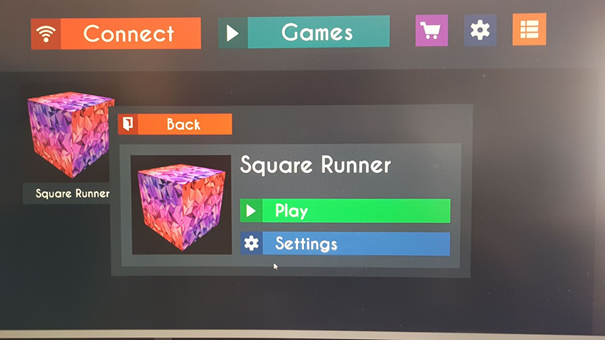
\includegraphics[scale=0.7]{images/design01.png} 
        \caption{Erster Shop Prototyp}
        \label{img:design01}
    \end{figure}
\end{center}
Für die ersten Iterationen des Projekts wählten wir dunkle Farben um auch das Spielen in den späteren Stunden zu ermöglichen. Die Grafik \ref{img:design01} zeigt das Server Interface, wobei hier das Shop-Interface zu sehen ist, sowie die Detailansicht eines Spieles. 
\newline
\begin{center}
    \begin{figure}
        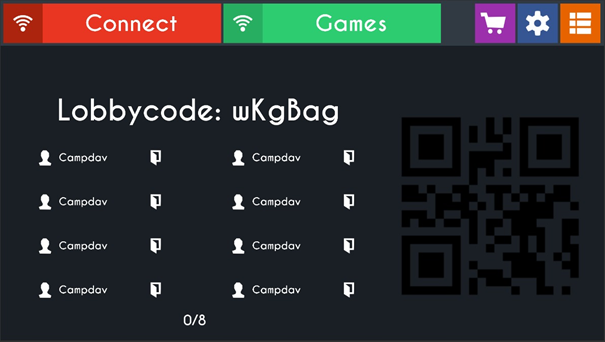
\includegraphics[scale=0.7]{images/design02.png} 
        \caption{Lobby Prototyp}
        \label{img:design02}
    \end{figure}
\end{center}
Um einerseits mehr Platz für den eigentlichen Inhalt zu haben und andererseits moderner auszusehen, änderten wir die Proportionen, die Abstände und Teils die Farben, um an die Kacheln von Windows 8, zu erinnern, wie in der Abbildung \ref{img:design02} zu sehen. Hier ist die Lobbyansicht ausgewählt. 
\newline
\begin{center}
    \begin{figure}
        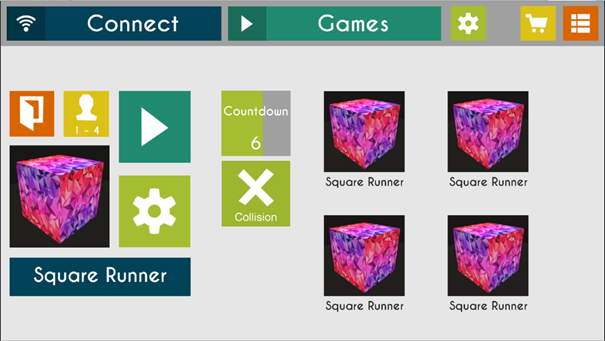
\includegraphics[scale=0.7]{images/design03.png} 
        \caption{Shopdetailansicht mit Einstellungen und hellem Farbschema}
        \label{img:design03}
    \end{figure}
\end{center}
Ludimus war Primär als Produkt für Familien mit Kindern gedacht. Dunkle Farben übermittelten nicht das Gefühl, das wir transportieren wollten, weshalb wir uns für helle Farben auf weißen Hintergrund entschieden. \ref{img:design03} zeigt auch eine Umgestaltung der Detailansicht, dazu jedoch in Punkt \ref{sec:shop} mehr.
\newline
\begin{center}
    \begin{figure}
        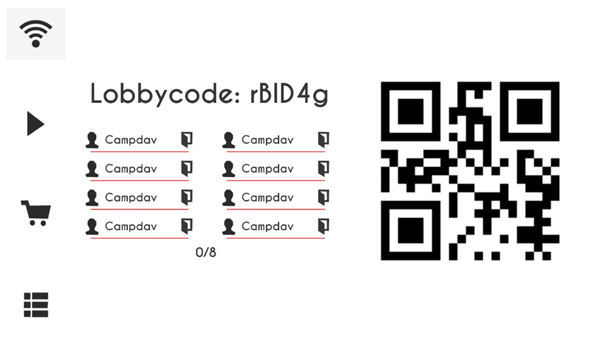
\includegraphics[scale=0.7]{images/design04.png} 
        \caption{Schwarz-Weiß Designentwurf}
        \label{img:design04}
    \end{figure}
\end{center}
Einen gewissen Rückschritt in Sachen Farben stellte unser nächstes UI dar, zu sehen in \ref{img:design04}. Der Hintergedanke hierbei war die Vereinfachung der Plattform und ein schwarz-weißes Design half uns dabei. Nutzer sahen nun auch erstmals, in welchem Menü sie sich befanden, da dieses nun einen dunkleren Hintergrund bekam. Globale Einstellungen für die Plattform selbst als eigener Punkt, wurden mit diesem Design entfernt.
\newline
\begin{center}
    \begin{figure}
        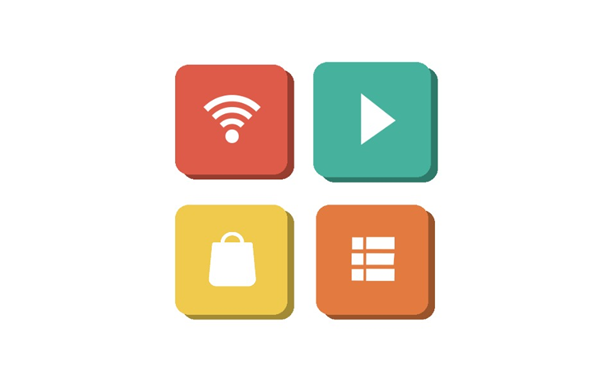
\includegraphics[scale=0.7]{images/design05.png}
        \caption{Buntes Hauptmenü mit Schatten und abgerundeten Ecken}
        \label{img:design05}
    \end{figure}
\end{center}
In den nächsten Iterationen brachten wir einerseits Farbe zurück, rundeten andererseits aber auch alle Buttons ab und gaben ihnen einen Schatten, wie in \ref{img:design05} zu sehen. Hatte man in allen bisherigen Versionen noch eine Menüleiste und einen Inhaltsteil, so entfernten wir Erstere um nur den Inhalt darstellen zu können. Drückt der Nutzer nun auf einen der vier Menüpunkte, so schwenkt die Kamera in dessen Ecke und der Inhalt wird dort angezeigt. Mit einem Zurück-Knopf kann der Benutzer anschließend wieder zum Hauptmenü gelangen. Wir implementierten zusätzlich noch eine Farbauswahl für das gesamte Interface. Benutzer konnten sich bestimmte Farbkombinationen auswählen, um sowohl die vier Primärfarben, als auch den Hintergrund zu ändern. Diese Entscheidungen hatten jedoch alle mehrere Nachteile, weshalb wir alles wieder verändern mussten. Die Kameraanimationen waren zwar interessant anzusehen, jedoch verlangsamten sie den Navigationsprozess Unnötigerweise. Zusätzliche Probleme machten verschiedene Formate, da die Animationen nur auf 16:9 optimiert waren. Obwohl das Farbschema wechseln gut funktioniert hat und Menschen mit verschiedenen Präferenzen die Möglichkeit gab das UI zu verändern, mussten wir das Feature entfernen, da uns die Erkennung unserer Marke wichtig war und wir erreichen wollten, dass sobald Familien unser Logo oder unsere Farben sehen an uns denken können. Wenn jeder seine eigenen Farben festlegen kann, ist dies nicht möglich.
\newline
Bisher waren eine Übersicht der Lobby, der Shop, alle Heruntergeladenen Spiele und ein Menü für Optionen in der Serveransicht und der Client konnte nur Name und Lobbycode eingeben und sich anschließend verbinden. Wollte eine Gruppe also spielen, mussten sich zuerst alle Spieler auf deren Handys zum großen Bildschirm verbinden und danach musste ein Spieler das Tablet, den Laptop oder den Fernseher bedienen um ein Spiel zu starten, oder zuerst herunterladen. Speziell beim Spielen im Wohnzimmer über den Fernseher gibt es hier enorme Probleme, die mit der Steuerung von Menüs mit der Fernbedienung zu tun haben. Um diese unnötige Interaktion mit dem großen Bildschirm zu entfernen, gestalteten wir die Aufteilung der Menüs komplett um. Der Server sollte nur noch die Lobby anzeigen, da diese keine Interaktion forderte. Sowohl Spielernamen, als auch der Lobbycode in schriftlicher und grafischer Form, konnten so größer dargestellt werden. Zusätzlich zu einem Login Fenster, welches wir bei App-Start dem Client hinzugefügt haben, wurden Spieler wie immer aufgefordert ihren Namen und den Lobbycode einzugeben um sich anschließend zu verbinden. Dieser Vorgang blieb für alle Spieler bis auf den ersten gleich. Dieser hat nun jedoch die Kontrolle über die Lobby und kann sowohl neue Spiele herunterladen, als auch bereits heruntergeladene Spiele starten. Um das Interface zu vereinfachen, vereinten wir den Shop mit den heruntergeladenen Spielen. Durch den Verzicht einer einheitlichen Trennung kann der Nutzer nicht unterscheiden ob ein Spiel zuerst heruntergeladen werden muss und probiert so viel mehr neue Spiele. Die Downloadzeit überschreitet nur selten 10 Sekunden, wodurch dies nur noch verstärkt wird. 
\newline
\begin{center}
    \begin{figure}
        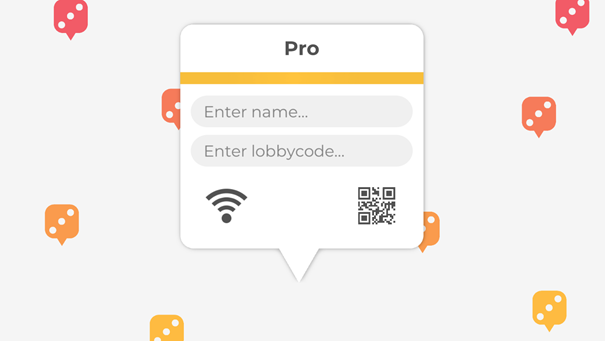
\includegraphics[scale=0.7]{images/design06.png} 
        \caption{UI zum Verbinden zu einer Lobby}
        \label{img:design06}
    \end{figure}
\end{center}
Wie in \ref{img:design06} zu sehen, ist unser Userinterface mit dem Ludimus Logo eng verknüpft, um es so in die Köpfe der Nutzer zu bekommen. Das UI zum Verbinden zu einer Lobby ist in eine Form, die dem Ludimus Logo ähnelt, eingebettet. Zusätzlich steigen im Hintergrund Ludimus Ballone auf, die ihre Farbe in Abhängigkeit des Subskription Levels, des eingeloggten Nutzers, ändern. 

\subsection{Spezielle Designentscheidungen} \label{sec:special-design}
\subsubsection{Shop} \label{sec:shop}
Der Shop änderte sich über die verschiedenen Versionen am meisten, da die richtige Präsentation der Spiele essentiell für den Kauf eines teureren Subskription Plans ist. Die Änderungen gliedern sich in die Anzeige aller Spiele und die Anzeige eines Spieles.
\newline
Zu Beginn wurden alle Spiele in einem Gitter mit Zeilen und Spalten angezeigt, wie in \ref{img:design01} zu sehen. Überlegungen bezüglich Sortierung oder Suche wurden zu diesem Zeitpunkt noch nicht angestellt. Um Nutzern zu ermöglichen nur Spiele einer bestimmten Art zu sehen, erweiterten wir deren Datenmodell um das Feld „Genre“. Zusätzlich vergaben wir einen Farbcode für jedes Genre, um dem Nutzer schnell ersichtlich zu machen um welche Art von Spiel es sich handelt. Da wir die Plattform für externe Entwickler öffnen wollten, um mehr Spiele anbieten zu können, fügten wir die Reiter „New“, „Top“ und „New Update“ hinzu. Der Gedanke hierbei war neue Spiele eine kurze Zeit unter  „New“ anzuzeigen und Spiele, die oft gespielt werden sollten anschließend unter „Top“ zu finden sein. Um auch ältere Spiele wieder beliebt zu machen oder Entwicklern eine zweite Chance geben zu können, falls der ursprüngliche Release nicht funktioniert hat, würden Spiele die neue Updates erhalten unter „New Update“ gezeigt werden. Den Plan externe Entwickler mit einzubeziehen verworfen wir jedoch, wodurch eine solche Gliederung nicht mehr nötig war, da zu wenig Spiele dafür verfügbar wären. Wie in Abbildung \ref{img:design07} zu sehen, vereinfachten wir zusätzlich die Anzeige der Spiele, in dem wir das Icon des Spieles größer machten, die Detailansicht hinter einem Menü versteckten und wir das Genre des Spieles durch die Farbe der Umrandung klar darstellten. Die zwei Eingabefelder, am unteren Ende des Bildschirms, mit dem Knopf in der Mitte gehören zum Debug Modus, der nur für Entwickler ist, dazu mehr in \ref{sec:debug-modus}.
\begin{center}
    \begin{figure}
        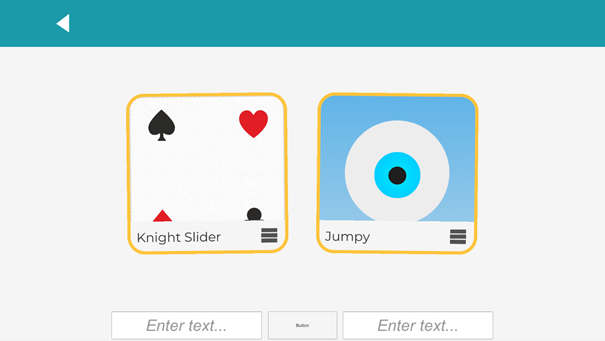
\includegraphics[scale=0.7]{images/design07.png} 
        \caption{Finale Shoppräsentation mit Debug Modus}
        \label{img:design07}
    \end{figure}
\end{center}
Die in Abbildung \ref{img:design03} zu sehenden spielspezifischen Einstellungen wurden entfernt und durch Optionenmenüs im Spiel selbst ersetzt. Durch Änderungen im Startprozess von Spielen wurden Spiele mit mehreren Szenen ermöglicht, wodurch die alte Methode überflüssig wurde.